%%%%%%%%%%%%%%%%%%%%%%%%%%%%%%%%%%%%%%%%%
% Jacobs Landscape Poster
% LaTeX Template
% Version 1.1 (14/06/14)
%
% Created by:
% Computational Physics and Biophysics Group, Jacobs University
% https://teamwork.jacobs-university.de:8443/confluence/display/CoPandBiG/LaTeX+Poster
% 
% Further modified by:
% Nathaniel Johnston (nathaniel@njohnston.ca)
%
% This template has been downloaded from:
% http://www.LaTeXTemplates.com
%
% License:
% CC BY-NC-SA 3.0 (http://creativecommons.org/licenses/by-nc-sa/3.0/)
%
%%%%%%%%%%%%%%%%%%%%%%%%%%%%%%%%%%%%%%%%%

%----------------------------------------------------------------------------------------
%	PACKAGES AND OTHER DOCUMENT CONFIGURATIONS
%----------------------------------------------------------------------------------------

\documentclass[final]{beamer}

\usepackage[scale=1.24]{beamerposter} % Use the beamerposter package for laying out the poster

\usetheme{confposter} % Use the confposter theme supplied with this template

\setbeamercolor{block title}{fg=ngreen,bg=white} % Colors of the block titles
\setbeamercolor{block body}{fg=black,bg=white} % Colors of the body of blocks
\setbeamercolor{block alerted title}{fg=white,bg=dblue!70} % Colors of the highlighted block titles
\setbeamercolor{block alerted body}{fg=black,bg=dblue!10} % Colors of the body of highlighted blocks
% Many more colors are available for use in beamerthemeconfposter.sty

%-----------------------------------------------------------
% Define the column widths and overall poster size
% To set effective sepwid, onecolwid and twocolwid values, first choose how many columns you want and how much separation you want between columns
% In this template, the separation width chosen is 0.024 of the paper width and a 4-column layout
% onecolwid should therefore be (1-(# of columns+1)*sepwid)/# of columns e.g. (1-(4+1)*0.024)/4 = 0.22
% Set twocolwid to be (2*onecolwid)+sepwid = 0.464
% Set threecolwid to be (3*onecolwid)+2*sepwid = 0.708

\newlength{\sepwid}
\newlength{\onecolwid}
\newlength{\twocolwid}
\newlength{\threecolwid}
\setlength{\paperwidth}{48in} % A0 width: 46.8in
\setlength{\paperheight}{36in} % A0 height: 33.1in
\setlength{\sepwid}{0.024\paperwidth} % Separation width (white space) between columns
\setlength{\onecolwid}{0.22\paperwidth} % Width of one column
\setlength{\twocolwid}{0.464\paperwidth} % Width of two columns
\setlength{\threecolwid}{0.708\paperwidth} % Width of three columns
\setlength{\topmargin}{-0.5in} % Reduce the top margin size


%-----------------------------------------------------------
\usepackage[most]{tcolorbox}
\usepackage{graphicx}  % Required for including images
\usepackage{adjustbox}
\usepackage{caption}
\usepackage{booktabs} % Top and bottom rules for tables
\usepackage{graphicx}
\usepackage{bbding}
\usepackage{pifont}
\usepackage{wasysym}
\usepackage{amssymb}
\newcommand{\xmark}{\text{\ding{55}}}
\usepackage{colortbl}

%------------------------------------------------------------
%   Headline Colours
%------------------------------------------------------------

%------------------------------------------------------------

%----------------------------------------------------------------------------------------
%	TITLE SECTION 
%----------------------------------------------------------------------------------------

\title{%
  \texorpdfstring{%
    \makebox[\linewidth]{%
      \makebox[0pt][l]{%
        \raisebox{\dimexpr-\height+\baselineskip}[0pt][0pt]
          {
\includegraphics[height=2\baselineskip]{figs/fsu-seal-gold.png}}% Left logo
      }\hfill
      \makebox[0pt]{Analyzing Hardware Parameters in GPU based HPC Platform}%
      \hfill\makebox[0pt][r]{%
        \raisebox{\dimexpr-\height+\baselineskip}[0pt][0pt]
          {
\includegraphics[height=2\baselineskip]{figs/fsu-seal-gold.png}}% Right logo
      }%
    }%
  }
  {Simulating Hardware Design Parameters for Future HPC Platform}}

\author{Saptarshi Bhowmik\textsuperscript{1}, Nikhil Jain\textsuperscript{2},, Abhinav Bhatele\textsuperscript{3} and Xin Yuan\textsuperscript{1}} % Author(s)

\institute{1. Florida State University, 2. NVIDIA, Inc, 3. University of Maryland} % Institution(s)

%----------------------------------------------------------------------------------------

\begin{document}

\addtobeamertemplate{block end}{}{\vspace*{2ex}} % White space under blocks
\addtobeamertemplate{block alerted end}{}{\vspace*{2ex}} % White space under highlighted (alert) blocks

\setlength{\belowcaptionskip}{2ex} % White space under figures
\setlength\belowdisplayshortskip{2ex} % White space under equations

\begin{frame}[t] % The whole poster is enclosed in one beamer frame

\begin{columns}[t] % The whole poster consists of three major columns, the second of which is split into two columns twice - the [t] option aligns each column's content to the top

\begin{column}{\sepwid}\end{column} % Empty spacer column

\begin{column}{\onecolwid} % The first column

%----------------------------------------------------------------------------------------
%	Goals
%----------------------------------------------------------------------------------------

\begin{alertblock}{Goals}
\begin{itemize}
\item \textbf{Use discrete-event simulations to study various hardware design parameters and their impact on the performance of HPC workloads}
\item \textbf{Study several parameters including nework bandwidth, number of GPUs per node  in the context of two most popular network topologies Fat-Tree and  1d-Dragonfly}
\end{itemize}
\end{alertblock}

%----------------------------------------------------------------------------------------
%	INTRODUCTION
%----------------------------------------------------------------------------------------
\vspace{-1em}
\begin{block}{Introduction}

Today's high-end HPC clusters employ many GPUs per node. The performance of applications on such a platform depends heavily on the interconnection network performance [1]. As such, it is important to understand the impact of hardware parameters on the overall application and system performance. In this research, we perform extensive simulation study to understand hardware parameters and their impact on the performance of HPC workload.


\end{block}
%----------------------------------------------------------------------------------------
%	METHODS
%----------------------------------------------------------------------------------------
\vspace{-1em}
\begin{block}{Method}
\textbf{System Configuration} 
\begin{itemize}
\item \textbf{Interconnection Network} Two network topology that is implemented in TraceR-CODES simulator, 1d - Dragonfly and Fat-Tree with Adaptive Routing.
\item \textbf{Number of GPU's per node} from 1-GPU/Node, 2-GPU/Node, 4-GPU/Node and 8-GPU/Node configuration.
\item \textbf{Link bandwidths} Base bandwidth x is 10 Gbps, from x/8, x/4, x/2, x, 2x, 4x, 8x bandwidths are used.
\end{itemize}
\begin{table}
\begin{adjustbox}{width=\columnwidth,left}

\begin{tabular}{|c|c|c|} \hline
\hline
\textbf{Traces} & \textbf{Computation Intensive} & \textbf{Communication Intensive} \\ \hline
\cellcolor{ProcessBlue!10}Stencil4d & \cellcolor{ProcessBlue!10}\xmark & \cellcolor{ProcessBlue!10}\CheckmarkBold  \\    \hline
Kripke & \CheckmarkBold & \xmark  \\    \hline
\cellcolor{ProcessBlue!10}Laghos & \cellcolor{ProcessBlue!10}\CheckmarkBold & \cellcolor{ProcessBlue!10}\xmark  \\    \hline
Subcomm-a2a & \xmark & \CheckmarkBold  \\    \hline
\cellcolor{ProcessBlue!10}Sw4lite & \cellcolor{ProcessBlue!10}\CheckmarkBold  & \cellcolor{ProcessBlue!10}\CheckmarkBold  \\    \hline
Amg & \CheckmarkBold  & \CheckmarkBold  \\    \hline
\end{tabular}
\end{adjustbox}


\caption{Application Traces}
\end{table}



\end{block}

%------------------------------------------------





%----------------------------------------------------------------------------------------

\end{column} % End of the first column

\begin{column}{\sepwid}\end{column} % Empty spacer column

\begin{column}{\twocolwid} % Begin a column which is two columns wide (column 2)

\begin{columns}[t,totalwidth=\twocolwid] % Split up the two columns wide column

\begin{column}{\onecolwid}\vspace{-.6in} % The first column within column 2 (column 2.1)
\vspace{-1em}
%----------------------------------------------------------------------------------------
%	Experimental Setup
%----------------------------------------------------------------------------------------

\begin{block}{Method}

We are running 20 Workloads of randomly selected jobs from the above application from ranks 32, 64, 128, 256 and 512. We make sure that each rank of an application appears atleast 4 times across all 20 workloads. 
\end{block}
%----------------------------------------------------------------------------------------

\end{column} % End of column 2.1

\begin{column}{\onecolwid}\vspace{-.6in} % The second column within column 2 (column 2.2)

%----------------------------------------------------------------------------------------
%	Results 2
%----------------------------------------------------------------------------------------
\vspace{-1em}
\begin{block}{Results}
%$\bullet$ We see that without scaling the Stencil and Subcom jobs are behaving well, with error percentage less than 20 percent, although the Kripke jobs show most variations.
%\vspace{\baselineskip}
\newline
\textbf{Second}, Impact of Bandwidth and different GPU's per node on Application Performance.

\begin{figure}
\centering
\begin{minipage}{1\textwidth}
\centering
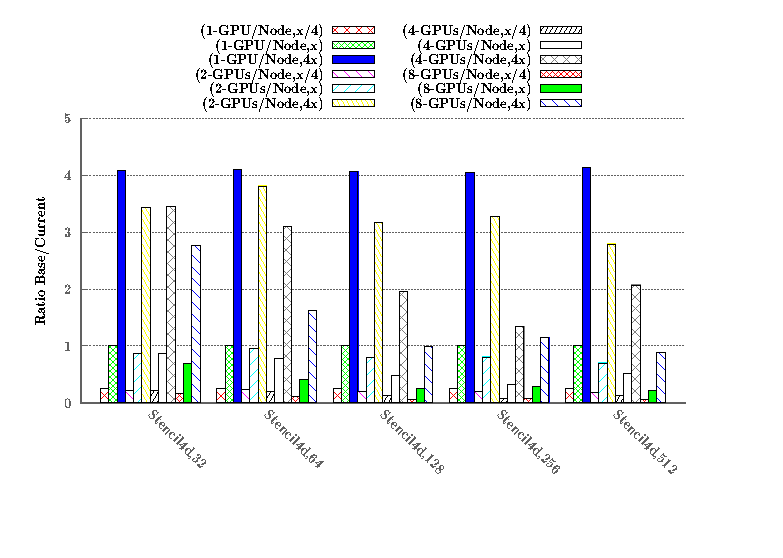
\includegraphics[width=1\linewidth, height=20cm]{figs/ftree-bw-mapping-comm-stencil.eps}
\captionsetup{labelformat=empty}
\caption{Ratio of Bandwidth,GPUs per node mapping for Stencil in Fat-Tree}
\end{minipage}
\end{figure}

\end{block}

%----------------------------------------------------------------------------------------

\end{column} % End of column 2.2

\end{columns} % End of the split of column 2 - any content after this will now take up 2 columns width


\begin{columns}[t,totalwidth=\twocolwid] % Split up the two columns wide column again

\begin{column}{\onecolwid} % The first column within column 2 (column 2.1)
\vspace{-1em}
%----------------------------------------------------------------------------------------
%	RESULTS 1
%----------------------------------------------------------------------------------------
\vspace{-2.5em}
\begin{block}{Results}
\textbf{First}, Impact of Number of GPU's per node on Application performance. 
\begin{figure}
\centering
\begin{minipage}{.45\textwidth}
\centering
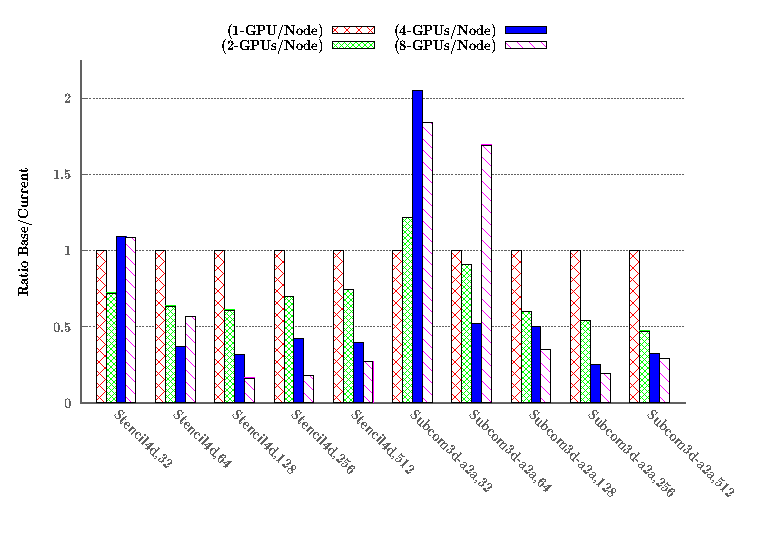
\includegraphics[width=1\linewidth]{figs/dfly-x-mapping-comm.eps}
\captionsetup{labelformat=empty}
\caption{Communication Apps}
\label{fig:13a}
\end{minipage}
\begin{minipage}{.45\textwidth}
\centering
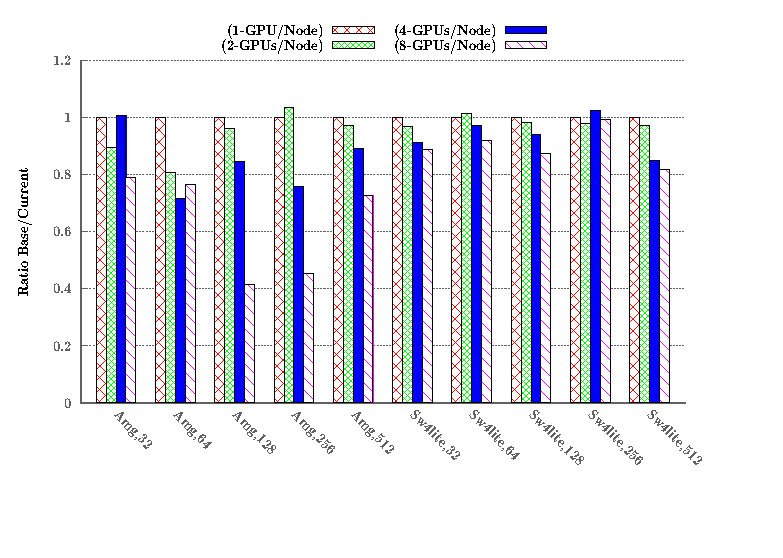
\includegraphics[width=1\linewidth]{figs/dfly-x-mapping-comp-new.eps}
\captionsetup{labelformat=empty}
\caption{Amg, Sw4lite Proxy}
\label{fig:13b}
\end{minipage}
\captionsetup{labelformat=empty}
\caption{1d-Dragonfly Topology}
\end{figure}

\begin{figure}
\centering
\begin{minipage}{.45\textwidth}
\centering
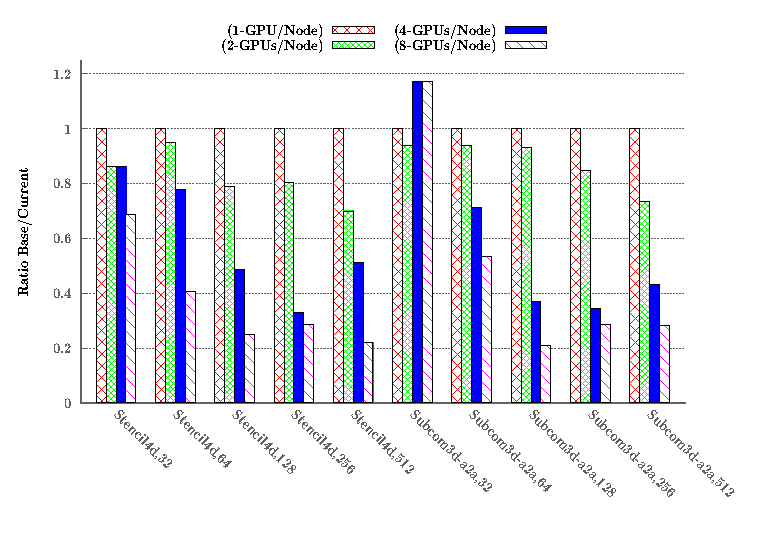
\includegraphics[width=1\linewidth]{figs/ftree-x-mapping-comm.eps}
\captionsetup{labelformat=empty}
\caption{Communication Apps}
\label{fig:13a}
\end{minipage}
\begin{minipage}{.45\textwidth}
\centering
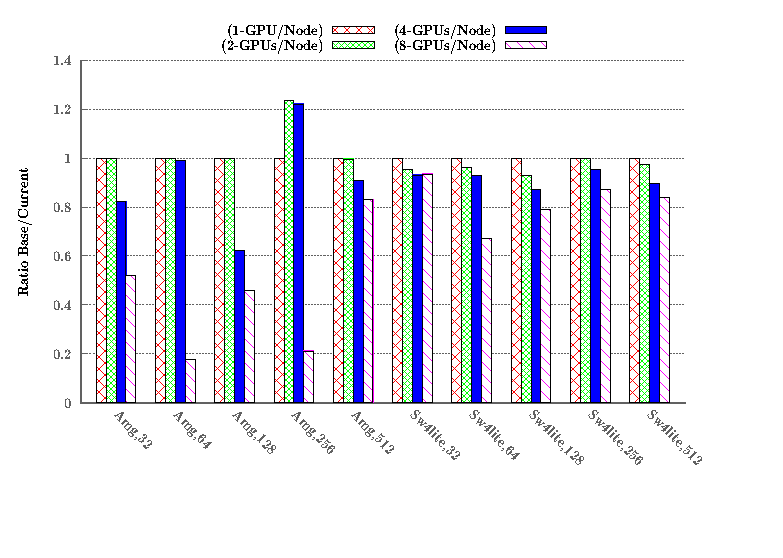
\includegraphics[width=1\linewidth]{figs/ftree-x-mapping-comp-new.eps}
\captionsetup{labelformat=empty}
\caption{Amg, Sw4lite Proxy}
\label{fig:13b}
\end{minipage}
\captionsetup{labelformat=empty}
\caption{Fat-Tree Topology}
\end{figure}


\begin{itemize}
\item \textbf{GPUs per node} The communication intensive applications slowdown when the number of GPUs per node is increased, among the proxy applications only AMG shows slowdown.
\end{itemize}
\end{block}

%----------------------------------------------------------------------------------------

\end{column} % End of column 2.1

\begin{column}{\onecolwid} % The second column within column 2 (column 2.2)
\vspace{-1em}
%----------------------------------------------------------------------------------------
%	RESULTS 
%----------------------------------------------------------------------------------------



\begin{figure}
\centering
\begin{minipage}{1\textwidth}
\centering
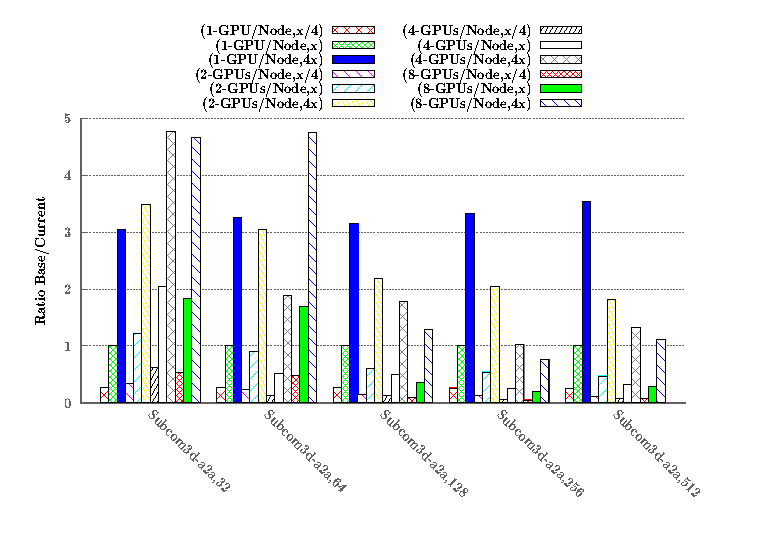
\includegraphics[width=1\linewidth, height=18cm]{figs/dfly-bw-mapping-comm-subcom.eps}
\captionsetup{labelformat=empty}
\caption{Ratio of Bandwidth,GPUs per node for Subcom3d-a2a in 1d-Dragonfly}
\end{minipage}
\end{figure}
\begin{figure}
\centering
\begin{minipage}{1\textwidth}
\centering
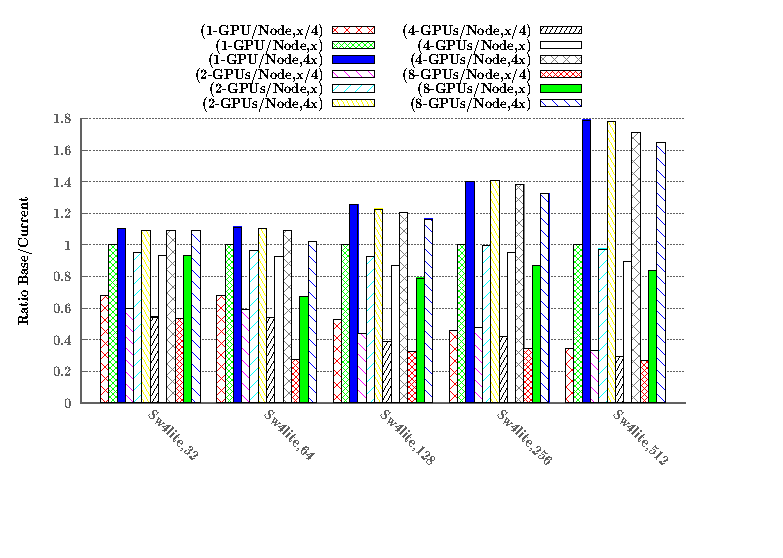
\includegraphics[width=1\linewidth, height=18cm]{figs/ftree-bw-mapping-comp-sw4lite.eps}
\captionsetup{labelformat=empty}
\caption{Ratio of Bandwidth,GPUs per node mapping for Sw4lite in Fat-Tree}
\end{minipage}
\end{figure}

%\begin{figure}
%\centering
%\begin{minipage}{.45\textwidth}
%\centering
%\includegraphics[width=1\linewidth]{full11.pdf}
%\captionsetup{labelformat=empty}
%\caption{Tapered Fat Tree Topology}
%\label{fig:13a}
%\end{minipage}
%\begin{minipage}{.45\textwidth}
%\centering
%\includegraphics[width=1\linewidth]{net11.pdf}
%\captionsetup{labelformat=empty}
%\caption{Quartz Topology}
%\label{fig:13b}
%\end{minipage}
%\captionsetup{labelformat=empty}
%\caption{Predicted Vs Observed time for Workload-1 1-Task/Node}
%\end{figure}

%\begin{figure}
%\begin{minipage}{.45\textwidth}
%\centering
%\includegraphics[width=1\linewidth]{full18.pdf}
%\captionsetup{labelformat=empty}
%\caption{Tapered Fat Tree Topology}
%\label{fig:13a}
%\end{minipage}
%\begin{minipage}{.45\textwidth}
%\centering
%\includegraphics[width=1\linewidth]{net18.pdf}
%\captionsetup{labelformat=empty}
%\caption{Quartz Topology}
%\label{fig:13b}
%\end{minipage}
%\captionsetup{labelformat=empty}
%\caption{Predicted Vs Observed time for Workload-1 8-Task/Node}
%\end{figure}





%----------------------------------------------------------------------------------------

\end{column} % End of column 2.2

\end{columns} % End of the split of column 2

\end{column} % End of the second column

\begin{column}{\sepwid}\end{column} % Empty spacer column

\begin{column}{\onecolwid} % The third column

%----------------------------------------------------------------------------------------
%	% CONCLUSION
%----------------------------------------------------------------------------------------

\begin{block}{Result}
\begin{itemize}

\item \textbf{Link Bandwidth} As we increase the number of GPU's per node. More bandwidth is needed to make the performance at par with lower GPU's per node configuration.
\vspace{\baselineskip}
\item In Subcom3d-a2a applications, applications with fewer ranks are performing better as more GPU's are mapped to one node, as there is more intra-node communication.
\end{itemize}
\end{block}



%----------------------------------------------------------------------------------------
%	FUTURE WORKS
%----------------------------------------------------------------------------------------

\begin{block}{Future Work}
\begin{itemize}
\item Every application has a sweet spot where the performance is the best, figure out the sweet spot for other HPC applications.
\vspace{\baselineskip}
\vspace{\baselineskip}
\item Try to study how other simulation environment and hardware design, such as NIC scheduling policies effect the performance of applications
\end{itemize}
\end{block}

%----------------------------------------------------------------------------------------
%	REFERENCES
%----------------------------------------------------------------------------------------

\begin{block}{References}

\nocite{*} % Insert publications even if they are not cited in the poster
\small{\bibliographystyle{unsrt}
\bibliography{sample}\vspace{0.55in}}
\vspace{-0.5em}
\small{\rmfamily{This work was performed under the auspices of the U.S. Department of Energy by Lawrence Livermore National Laboratory under Contract DE-AC52-07NA27344 (LLNL-POST-783752).}} 
\end{block}

%----------------------------------------------------------------------------------------

\end{column} % End of the third column

\end{columns} % End of all the columns in the poster

\end{frame} % End of the enclosing frame

\end{document}
